\documentclass[11pt,a4paper]{article}

\usepackage[margin=1in]{geometry}
\usepackage[T1]{fontenc}
\usepackage[utf8]{inputenc}
\usepackage{lmodern}
\usepackage{amsmath,amssymb}
\usepackage{graphicx}
\usepackage{booktabs}
\usepackage[authoryear,round]{natbib}
\usepackage{url}
\usepackage[hidelinks]{hyperref}
\usepackage[capitalise,noabbrev]{cleveref}
\usepackage{microtype}
\setlength{\emergencystretch}{2em}

\newcommand{\EQ}{\textsc{Eq}}
\newcommand{\FWD}{\textsc{Fwd}}
\newcommand{\BWD}{\textsc{Bwd}}
\newcommand{\NEG}{\textsc{Neg}}
\DeclareMathOperator{\rev}{rev}

\title{Directional Consistency in Fine-Grained NLI:\\
Baselines for DiCo-NLI (Track~1)\\[4pt]
\large CS-878 Deep Learning, Assignment 1}
\author{Muneeb Baig\\ MS Data Science, SEECS, NUST}
\date{October 2026}

\begin{document}
\maketitle

\section{Introduction and Task Definition}
\label{sec:intro}

NLI models can score well by exploiting superficial cues \citep{gururangan2018annotation}, and standard evaluation scores each ordered pair on its own, so it cannot show whether a model stays coherent when a pair is reversed. DiCo-NLI (SemEval-2027 Task~2) measures both \citep{diconli2026}. We work on Track~1 (English).

\paragraph{Black-box view.} The input is an ordered pair of short phrases $(t_1,t_2)$ and the output is one of four labels: \texttt{EQUIVALENCE} (\EQ), \texttt{FORWARD\_ENTAILMENT} (\FWD), \texttt{BACKWARD\_ENTAILMENT} (\BWD) or \texttt{NEGATIVE\_OTHER} (\NEG). \EQ{} means each phrase entails the other, \FWD{} that only $t_1\Rightarrow t_2$, \BWD{} that only $t_2\Rightarrow t_1$, and \NEG{} collects every other relation. For example, ``Japanese PM Shinzo Abe'' $\rightarrow$ ``Abe'' is \FWD, and the reversed pair is \BWD. A coherent classifier should therefore satisfy $f(t_2,t_1)=\rev(f(t_1,t_2))$, with $\rev(\FWD)=\BWD$, $\rev(\BWD)=\FWD$ and $\rev(\EQ)=\EQ$. \NEG{} rows appear in one orientation only.

\paragraph{White-box view.} \FWD{} and \BWD{} differ only in direction, so symmetric signals such as word overlap or cosine similarity cannot separate them. Similarity is also not equivalence: ``A sheep'' and ``A large sheep'' share almost everything but the relation is one-way. \NEG{} merges several relations, and the phrases are so short that one modifier often decides the label. There is also an obvious shortcut risk: the more specific phrase is usually longer, so a model could follow length instead of meaning.

\paragraph{Research question and hypotheses.} How far do shallow cues and standard fine-tuned encoders get on DiCo-NLI, and how much does consistency reflect correct classification? \textbf{H1:} surface cues such as length give non-trivial accuracy and high SoftCons. \textbf{H2:} fine-tuned cross-encoders beat the classical baselines on W-F1 and HardCons. \textbf{H3:} their remaining errors sit at the \NEG{} boundary rather than on direction.

\section{Related Work}
\label{sec:related}

\citet{gururangan2018annotation} showed that hypothesis-only classifiers reach about 67\% on SNLI and 53\% on MultiNLI, well above chance; our length-only and overlap-only probes apply the same idea to phrase pairs. DiCo-NLI is built from PhrasIS \citep{lopezgazpio2024phrasis}, over 10{,}000 expert-annotated phrase pairs from captions and headlines, and keeps only the reversible relations, mapping the rest to \NEG{} \citep{diconli2026}. Language models often fail to retrieve a fact backwards \citep[the Reversal Curse;][]{berglund2024reversal}, though BERT was unaffected in the setting of \citet{wu2024reversal}; DiCo-NLI asks the narrower question of whether a predicted relation transforms correctly under reversal. Its direct predecessor is \citet{apaolaza2026assessing}, who defined soft and hard coherence (the basis of SoftCons and HardCons) on PhrasIS, found encoders strongest among 17 models, linked errors to lexical overlap and prepositions, and warned that a model can be consistently wrong.

\section{Dataset}
\label{sec:dataset}

We use the official split: 3{,}042 training rows (1{,}760 \texttt{pair\_id}s) and 660 development rows (383 pairs). No \texttt{pair\_id} appears in both splits, so a reversed training pair cannot leak into development. Seven development rows still have an exact text match in training, which we treat as a limitation. Labels are similar in both splits: \FWD{} and \BWD{} about 29\% each, \EQ{} 26\% and \NEG{} 16\%. Because \NEG{} is the smallest class, we also report Macro F1.

\section{Exploratory Data Analysis}
\label{sec:eda}

The full plots are in the separate EDA file; below are the findings that shaped the models.

\textbf{Length.} In \FWD{} rows $t_1$ averages 3.58 tokens against 2.44 for $t_2$, and 77\% put the longer phrase first; \BWD{} mirrors this and \EQ/\NEG{} centre on zero (\cref{fig:length}, left). Length is a real directional signal, but a surface one, so we test it alone as a shortcut.

\textbf{Overlap and containment.} In 45\% of entailment rows one phrase's words are fully contained in the other (\cref{fig:length}, right). Mean Jaccard is 0.41 for entailment but only 0.24 for \EQ, because paraphrases use different words. Jaccard is symmetric, so we separate it from directional containment features.

\textbf{POS.} Words found only in $t_1$ of \FWD{} pairs are often adjectives (0.39 per pair vs.\ 0.16 for \EQ) and proper nouns, i.e.\ the details that make a phrase more specific. We add POS counts of non-shared words.

\textbf{Similarity and vocabulary.} MiniLM cosine is about 0.74 for entailment, 0.72 for \EQ{} and 0.62 for \NEG: it separates related from unrelated pairs but is direction-blind, so the encoders must read the pair jointly. 47\% of training word types occur once and 15.4\% of development tokens are unseen, which favours pretrained subword models over TF--IDF.

\begin{figure}[t]
\centering
\includegraphics[page=2,width=0.49\linewidth]{figures/eda_plots.pdf}\hfill
\includegraphics[page=5,width=0.49\linewidth]{figures/eda_plots.pdf}
\caption{Left: signed token-length difference $L(t_1)-L(t_2)$ per label. Right: word-set containment pattern per label (row-normalised).}
\label{fig:length}
\end{figure}

\section{Feature Engineering}
\label{sec:features}

From the EDA we build 26 features per ordered pair: length (token counts and signed token/character differences), symmetric overlap (Jaccard, identical text), directional coverage and containment in both directions, negation and digit mismatch, and spaCy POS counts (noun, proper noun, adjective, verb, preposition, number) of non-shared words on each side. All of them except Jaccard and the identical-text flag change sign or swap roles under reversal. Features are $z$-scored on the training set.

\section{Baseline Models}
\label{sec:baselines}

\textbf{Baseline A (classical).} Logistic regression (scikit-learn, $C=1$) on: length features only; symmetric overlap only, a probe that has no notion of direction; all 26 features; TF--IDF unigrams and bigrams computed separately for each phrase and concatenated so that order is kept; and TF--IDF plus features. A majority-class model gives the floor.

\textbf{Baseline B (fine-tuned encoders).} \texttt{bert-base-uncased} and \texttt{roberta-base} are fine-tuned end to end as cross-encoders that read $t_1$ and $t_2$ together, BERT with segment IDs. We use AdamW (lr $3\times10^{-5}$, weight decay 0.01), batch 16, linear warm-up, six epochs, and keep the final epoch by a rule fixed in advance. Each model is run with three seeds (13, 42, 87) on an Apple M4 GPU. An early BERT run dropped \texttt{token\_type\_ids}; after the fix the setup was frozen.

\section{Evaluation Setup}
\label{sec:evaluation}

We use the organisers' scorer on the 660 development rows, of which 554 form $M=277$ reversible pairs. Weighted F1 averages per-class F1 by class support; Macro F1 weights classes equally. For pair $i$ with predictions $\hat y_{i,1},\hat y_{i,2}$ and gold labels $y_{i,1},y_{i,2}$:
\begin{gather*}
\mathrm{SoftCons}=\frac{1}{M}\sum_{i=1}^{M} \mathbb{1}\big[\hat y_{i,1}\neq\NEG \wedge \hat y_{i,2}=\rev(\hat y_{i,1})\big],\\
\mathrm{HardCons}=\frac{1}{M}\sum_{i=1}^{M} \mathbb{1}\big[\hat y_{i,1}=y_{i,1}\wedge \hat y_{i,2}=y_{i,2}\big].
\end{gather*}
SoftCons ignores the gold labels, so a model can be consistent and wrong; HardCons requires both directions to be correct, so HardCons $\le$ SoftCons.

\section{Results}
\label{sec:results}

\begin{table}[t]
\centering
\small
\resizebox{\linewidth}{!}{%
\begin{tabular}{lccccc}
\toprule
Model & W-F1 & SoftCons & HardCons & Macro-F1 & Acc. \\
\midrule
Majority class & 0.129 & 0.000 & 0.000 & 0.112 & 0.288 \\
LR (length only) & 0.464 & \textbf{0.989} & 0.628 & 0.408 & 0.532 \\
LR (symmetric overlap only) & 0.324 & 0.368 & 0.188 & 0.291 & 0.370 \\
LR (engineered features) & 0.593 & 0.877 & 0.653 & 0.558 & 0.602 \\
TF--IDF + LR & 0.484 & 0.877 & 0.542 & 0.452 & 0.500 \\
TF--IDF + features + LR & 0.620 & 0.856 & 0.661 & 0.588 & 0.626 \\
\midrule
BERT-base (3 seeds) & 0.705 $\pm$ 0.023 & 0.774 $\pm$ 0.016 & 0.693 $\pm$ 0.021 & 0.680 $\pm$ 0.024 & 0.707 $\pm$ 0.020 \\
RoBERTa-base (3 seeds) & \textbf{0.765} $\pm$ 0.002 & 0.804 $\pm$ 0.011 & \textbf{0.739} $\pm$ 0.006 & \textbf{0.742} $\pm$ 0.002 & \textbf{0.762} $\pm$ 0.004 \\
\bottomrule
\end{tabular}}
\caption{Development-set results with the official scorer. W-F1, SoftCons and HardCons are the official metrics.}
\label{tab:results}
\end{table}

\Cref{tab:results} gives the main picture. With just four length features, LR reaches 0.464 W-F1 but an almost perfect 0.989 SoftCons. The symmetric-overlap probe, blind to direction, manages only 0.368 SoftCons. Directional features lift W-F1 to 0.593, and adding TF--IDF gives the best classical model (0.620). Both encoders are clearly better, and RoBERTa ($0.765\pm0.002$ W-F1) is also far more stable across seeds than BERT. The biggest per-class gain is on \EQ{} (F1 0.515 $\rightarrow$ 0.725 for RoBERTa), which fits the EDA: paraphrases share few words, so they need the lexical knowledge that pretraining brings. \NEG{} stays the weakest class for every model. Note also that the encoders have \emph{lower} SoftCons than the classical feature models (0.774--0.804 vs.\ 0.856--0.877) but \emph{higher} HardCons. \Cref{fig:curves} shows the training runs: loss keeps falling, while development W-F1 levels off after three or four epochs, so the final-epoch rule costs little.

\begin{figure}[t]
\centering
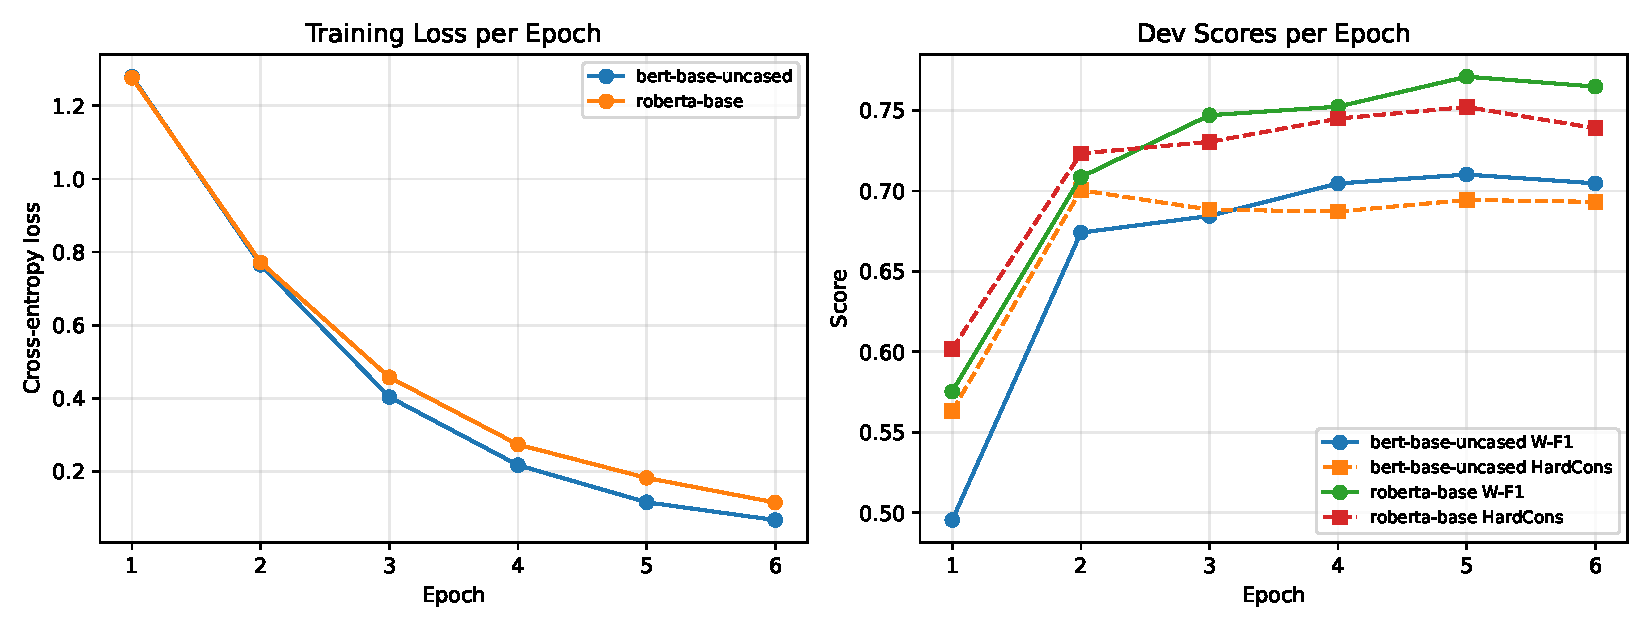
\includegraphics[width=\linewidth]{figures/training_curves.pdf}
\caption{Training loss (left) and development W-F1 and HardCons (right) per epoch, averaged over three seeds. Not used for model selection.}
\label{fig:curves}
\end{figure}

\section{Error Analysis}
\label{sec:errors}

\Cref{tab:pairs} splits the 277 reversible pairs by joint outcome (seed~42 encoders vs.\ the best classical model).

\begin{table}[t]
\centering
\small
\begin{tabular}{lccc}
\toprule
Outcome & TF--IDF + feats & BERT & RoBERTa \\
\midrule
Both directions correct & 183 & 186 & \textbf{204} \\
Consistent but wrong & \textbf{54} & 28 & 16 \\
Same entailment label both ways & 4 & 4 & 0 \\
\NEG{} in one direction only & 35 & 47 & 42 \\
Other inconsistency & 1 & 12 & 15 \\
\bottomrule
\end{tabular}
\caption{Outcomes for the 277 reversible development pairs (encoders: seed 42).}
\label{tab:pairs}
\end{table}

\begin{figure}[t]
\centering
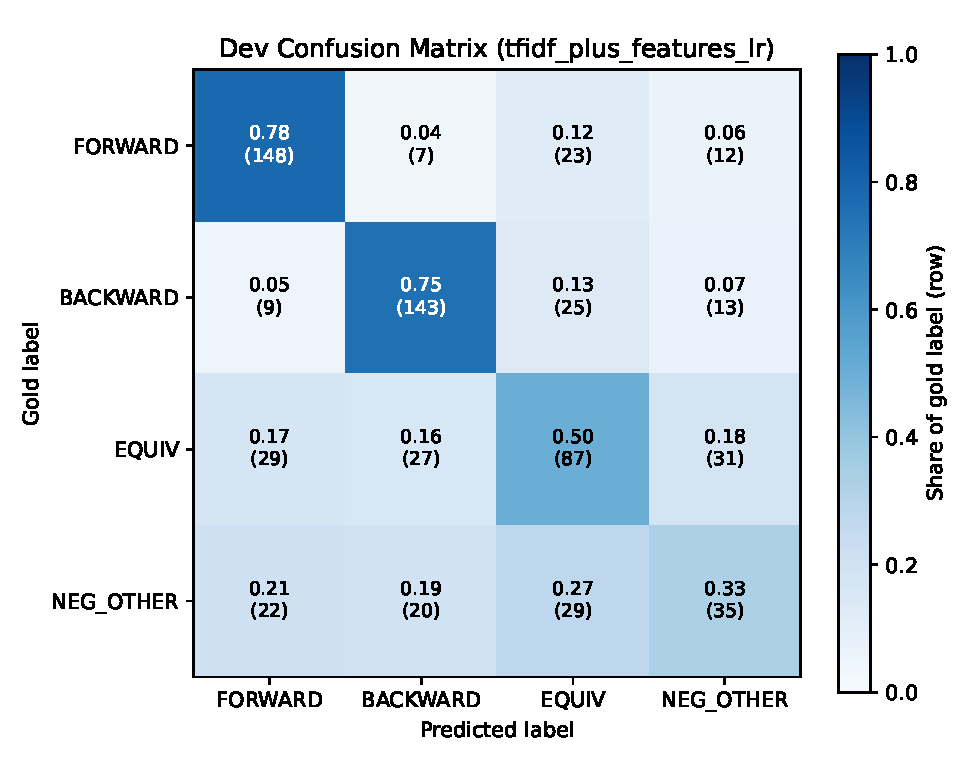
\includegraphics[width=0.49\linewidth]{figures/confusion_tfidf.pdf}\hfill
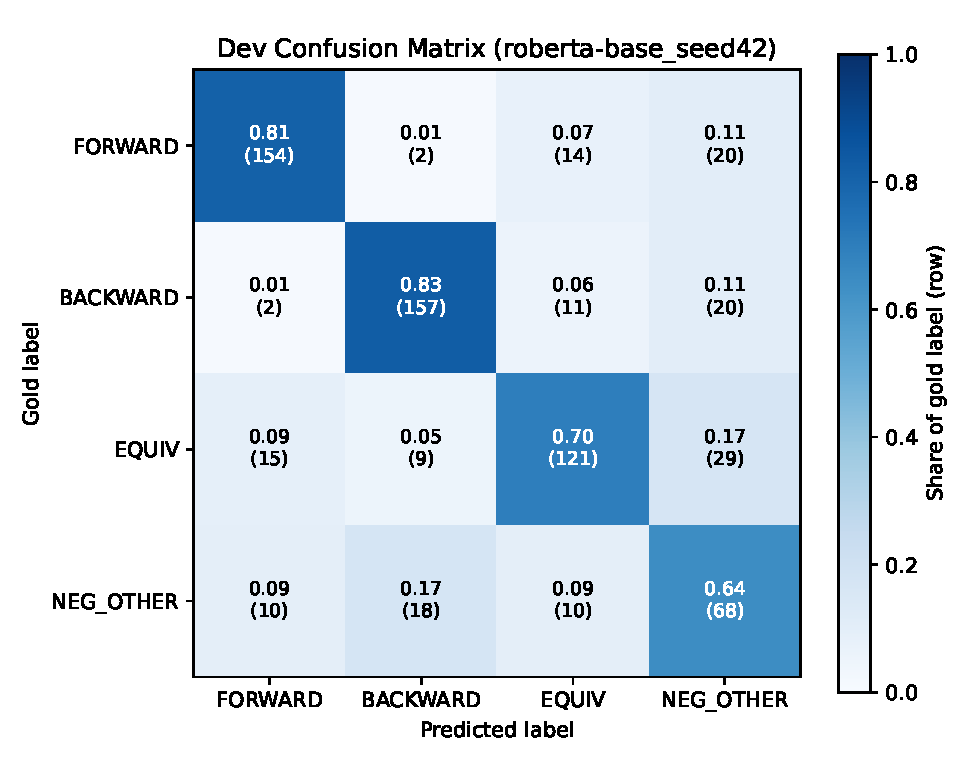
\includegraphics[width=0.49\linewidth]{figures/confusion_roberta.pdf}
\caption{Row-normalised development confusion matrices: TF--IDF + features LR (left) and RoBERTa-base, seed 42 (right).}
\label{fig:confusion}
\end{figure}

Much of the classical model's consistency is consistent wrongness (54 pairs). RoBERTa has only 16 such pairs and confuses \FWD{} with \BWD{} just twice each way, against 7 and 9 times for the classical model (\cref{fig:confusion}); its errors sit in the \NEG{} row and column instead. Its main problem is predicting \NEG{} for one orientation only (42 pairs), which is exactly why its SoftCons is lower. ``same-sex marriage'' / ``gay marriage'' is \EQ, but the length-only model, the best classical model and RoBERTa all predict \FWD/\BWD: consistent, and wrong. ``a monochrome photograph'' / ``a black and white photo'' splits the models: TF--IDF plus features gives \BWD/\FWD, BERT gives \EQ/\NEG, and only RoBERTa gets \EQ{} both ways. And in RoBERTa's largest error group, related pairs rejected as \NEG{} (69 rows), we find near-paraphrases such as ``martial arts clubs'' / ``Martial Arts Schools''. As in \citet{apaolaza2026assessing}, prepositions also cause errors. Finally, BERT without segment IDs gave the same label to both orientations in 119 of 190 entailment pairs, and in none once they were restored.

\section{Discussion}
\label{sec:discussion}

All three hypotheses are supported. Length alone produced near-perfect consistency with mediocre classification (H1); RoBERTa clearly beat the classical baselines on W-F1 and HardCons (H2); and the encoders largely solved direction, leaving the \NEG{} boundary as the main failure (H3). The clearest lesson is that SoftCons cannot be read as correctness: the most consistent model in the study is the one that only looks at phrase length.

\paragraph{Limitations.} We evaluate on the public development split (seven rows overlap with training) and did no hyperparameter search. MPS training is not fully deterministic (up to 0.03 W-F1 between identical runs), hence three seeds. Error categories come from heuristic rules, some gold labels are arguable (``Australian senator'' / ``Australian lawmaker'' is \NEG), and DeBERTa-v3 was dropped after NaN losses on MPS.

\section{Next Steps}
\label{sec:next}

The one-sided \NEG{} errors call for predicting both orientations jointly, or for training with a loss that rewards $f(t_2,t_1)=\rev(f(t_1,t_2))$, in the spirit of reverse training \citep{golovneva2024reverse}. We also plan class weighting for \NEG, a DeBERTa-v3 run on CUDA, and a blind test submission.

\bibliographystyle{plainnat}
\bibliography{references}

\end{document}
